% Options for packages loaded elsewhere
\PassOptionsToPackage{unicode}{hyperref}
\PassOptionsToPackage{hyphens}{url}
\PassOptionsToPackage{dvipsnames,svgnames*,x11names*}{xcolor}
%
\documentclass[
  12pt,
]{book}
\usepackage{amsmath,amssymb}
\usepackage{lmodern}
\usepackage{ifxetex,ifluatex}
\ifnum 0\ifxetex 1\fi\ifluatex 1\fi=0 % if pdftex
  \usepackage[T1]{fontenc}
  \usepackage[utf8]{inputenc}
  \usepackage{textcomp} % provide euro and other symbols
\else % if luatex or xetex
  \usepackage{unicode-math}
  \defaultfontfeatures{Scale=MatchLowercase}
  \defaultfontfeatures[\rmfamily]{Ligatures=TeX,Scale=1}
\fi
% Use upquote if available, for straight quotes in verbatim environments
\IfFileExists{upquote.sty}{\usepackage{upquote}}{}
\IfFileExists{microtype.sty}{% use microtype if available
  \usepackage[]{microtype}
  \UseMicrotypeSet[protrusion]{basicmath} % disable protrusion for tt fonts
}{}
\makeatletter
\@ifundefined{KOMAClassName}{% if non-KOMA class
  \IfFileExists{parskip.sty}{%
    \usepackage{parskip}
  }{% else
    \setlength{\parindent}{0pt}
    \setlength{\parskip}{6pt plus 2pt minus 1pt}}
}{% if KOMA class
  \KOMAoptions{parskip=half}}
\makeatother
\usepackage{xcolor}
\IfFileExists{xurl.sty}{\usepackage{xurl}}{} % add URL line breaks if available
\IfFileExists{bookmark.sty}{\usepackage{bookmark}}{\usepackage{hyperref}}
\hypersetup{
  pdftitle={Resources},
  pdfauthor={Noushin Nabavi \& Monica Granados},
  colorlinks=true,
  linkcolor=Maroon,
  filecolor=Maroon,
  citecolor=Blue,
  urlcolor=Blue,
  pdfcreator={LaTeX via pandoc}}
\urlstyle{same} % disable monospaced font for URLs
\usepackage{longtable,booktabs,array}
\usepackage{calc} % for calculating minipage widths
% Correct order of tables after \paragraph or \subparagraph
\usepackage{etoolbox}
\makeatletter
\patchcmd\longtable{\par}{\if@noskipsec\mbox{}\fi\par}{}{}
\makeatother
% Allow footnotes in longtable head/foot
\IfFileExists{footnotehyper.sty}{\usepackage{footnotehyper}}{\usepackage{footnote}}
\makesavenoteenv{longtable}
\usepackage{graphicx}
\makeatletter
\def\maxwidth{\ifdim\Gin@nat@width>\linewidth\linewidth\else\Gin@nat@width\fi}
\def\maxheight{\ifdim\Gin@nat@height>\textheight\textheight\else\Gin@nat@height\fi}
\makeatother
% Scale images if necessary, so that they will not overflow the page
% margins by default, and it is still possible to overwrite the defaults
% using explicit options in \includegraphics[width, height, ...]{}
\setkeys{Gin}{width=\maxwidth,height=\maxheight,keepaspectratio}
% Set default figure placement to htbp
\makeatletter
\def\fps@figure{htbp}
\makeatother
\setlength{\emergencystretch}{3em} % prevent overfull lines
\providecommand{\tightlist}{%
  \setlength{\itemsep}{0pt}\setlength{\parskip}{0pt}}
\setcounter{secnumdepth}{5}
\usepackage{booktabs}
\ifluatex
  \usepackage{selnolig}  % disable illegal ligatures
\fi
\usepackage[]{natbib}
\bibliographystyle{plainnat}

\title{Resources}
\author{Noushin Nabavi \& Monica Granados}
\date{2021-02-13}

\begin{document}
\maketitle

{
\hypersetup{linkcolor=}
\setcounter{tocdepth}{1}
\tableofcontents
}
\listoftables
\listoffigures
\hypertarget{preface}{%
\chapter{Preface}\label{preface}}

A repository to house materials for a open and reproducible workflows in the public service workshop.

The goal of this workshop is to introduce participants to concepts of \texttt{reproducible\ research}.
Reproducible research is the idea that data analyses, and more generally, scientific claims, are published with their data and software code so that others may verify the findings and build upon them.

This workshop focuses on the concepts and tools behind reporting modern data analyses in a reproducible manner. As part of this, we introduce tools that enable publishing data analyses in a single document that allows others to easily execute the same analysis to obtain the same results.

Additionally, as part of this workshop, we briefly introduce working with \texttt{R} and Rstudio to create a Rmarkdown document. R is a popular statistical computing language, commonly used in many scientific disciplines for statistical analysis, generating production-quality graphics, and automating data workflow tasks.

This work is licensed under the Creative Commons Attribution 4.0 International License.
To view a copy of this license, visit \url{http://creativecommons.org/licenses/by/4.0/}.

\hypertarget{learning-goals}{%
\section{Learning goals}\label{learning-goals}}

By the end of this workshop, EW2 participants will learn be able to:\\
- Define reproducible research and open workflows
- Discuss current issues surrounding reproducibility
- Discuss solutions and important components of reproducibility
- Identify tools that are used for reproducible and open research

In the demonstration part of the workshop, we will:

\begin{itemize}
\tightlist
\item
  Write basic markdown documents\\
\item
  Use knitr, rmarkdown and bookdown R packages to build various document types (e.g.~PDF, HTML and DOCX)\\
\item
  Create reproducible rmarkdown documents leveraging .Rproj and .RData\\
\item
  Create presentations from Rmarkdown documents that include R code\\
\item
  Work with git version control tools\\
\item
  Create reproducible and ``backed up'' analysis via remote repositories (e.g github)
\end{itemize}

\hypertarget{introduction-to-reproducible-research}{%
\chapter{Introduction to reproducible research}\label{introduction-to-reproducible-research}}

The terms \texttt{reproducible\ research} was coined by Jon Claerbout in the 1980s when he writes an essay on \href{http://sepwww.stanford.edu/sep/jon/reproducible.html}{reproducible} computational research, and describes the hurdles he faces when making a text book that incorporates text, data, and results in a stand-alone document. According to Claerbout's principle, `scholarship does not only consist of theorems and proofs but also and perhaps even more important of data, computer code and a runtime environment which provides readers with the possibility to reproduce all tables and figures in an article'.

This image by The Turing Way is a great representation of what Jon Claerbout may have had in mind:

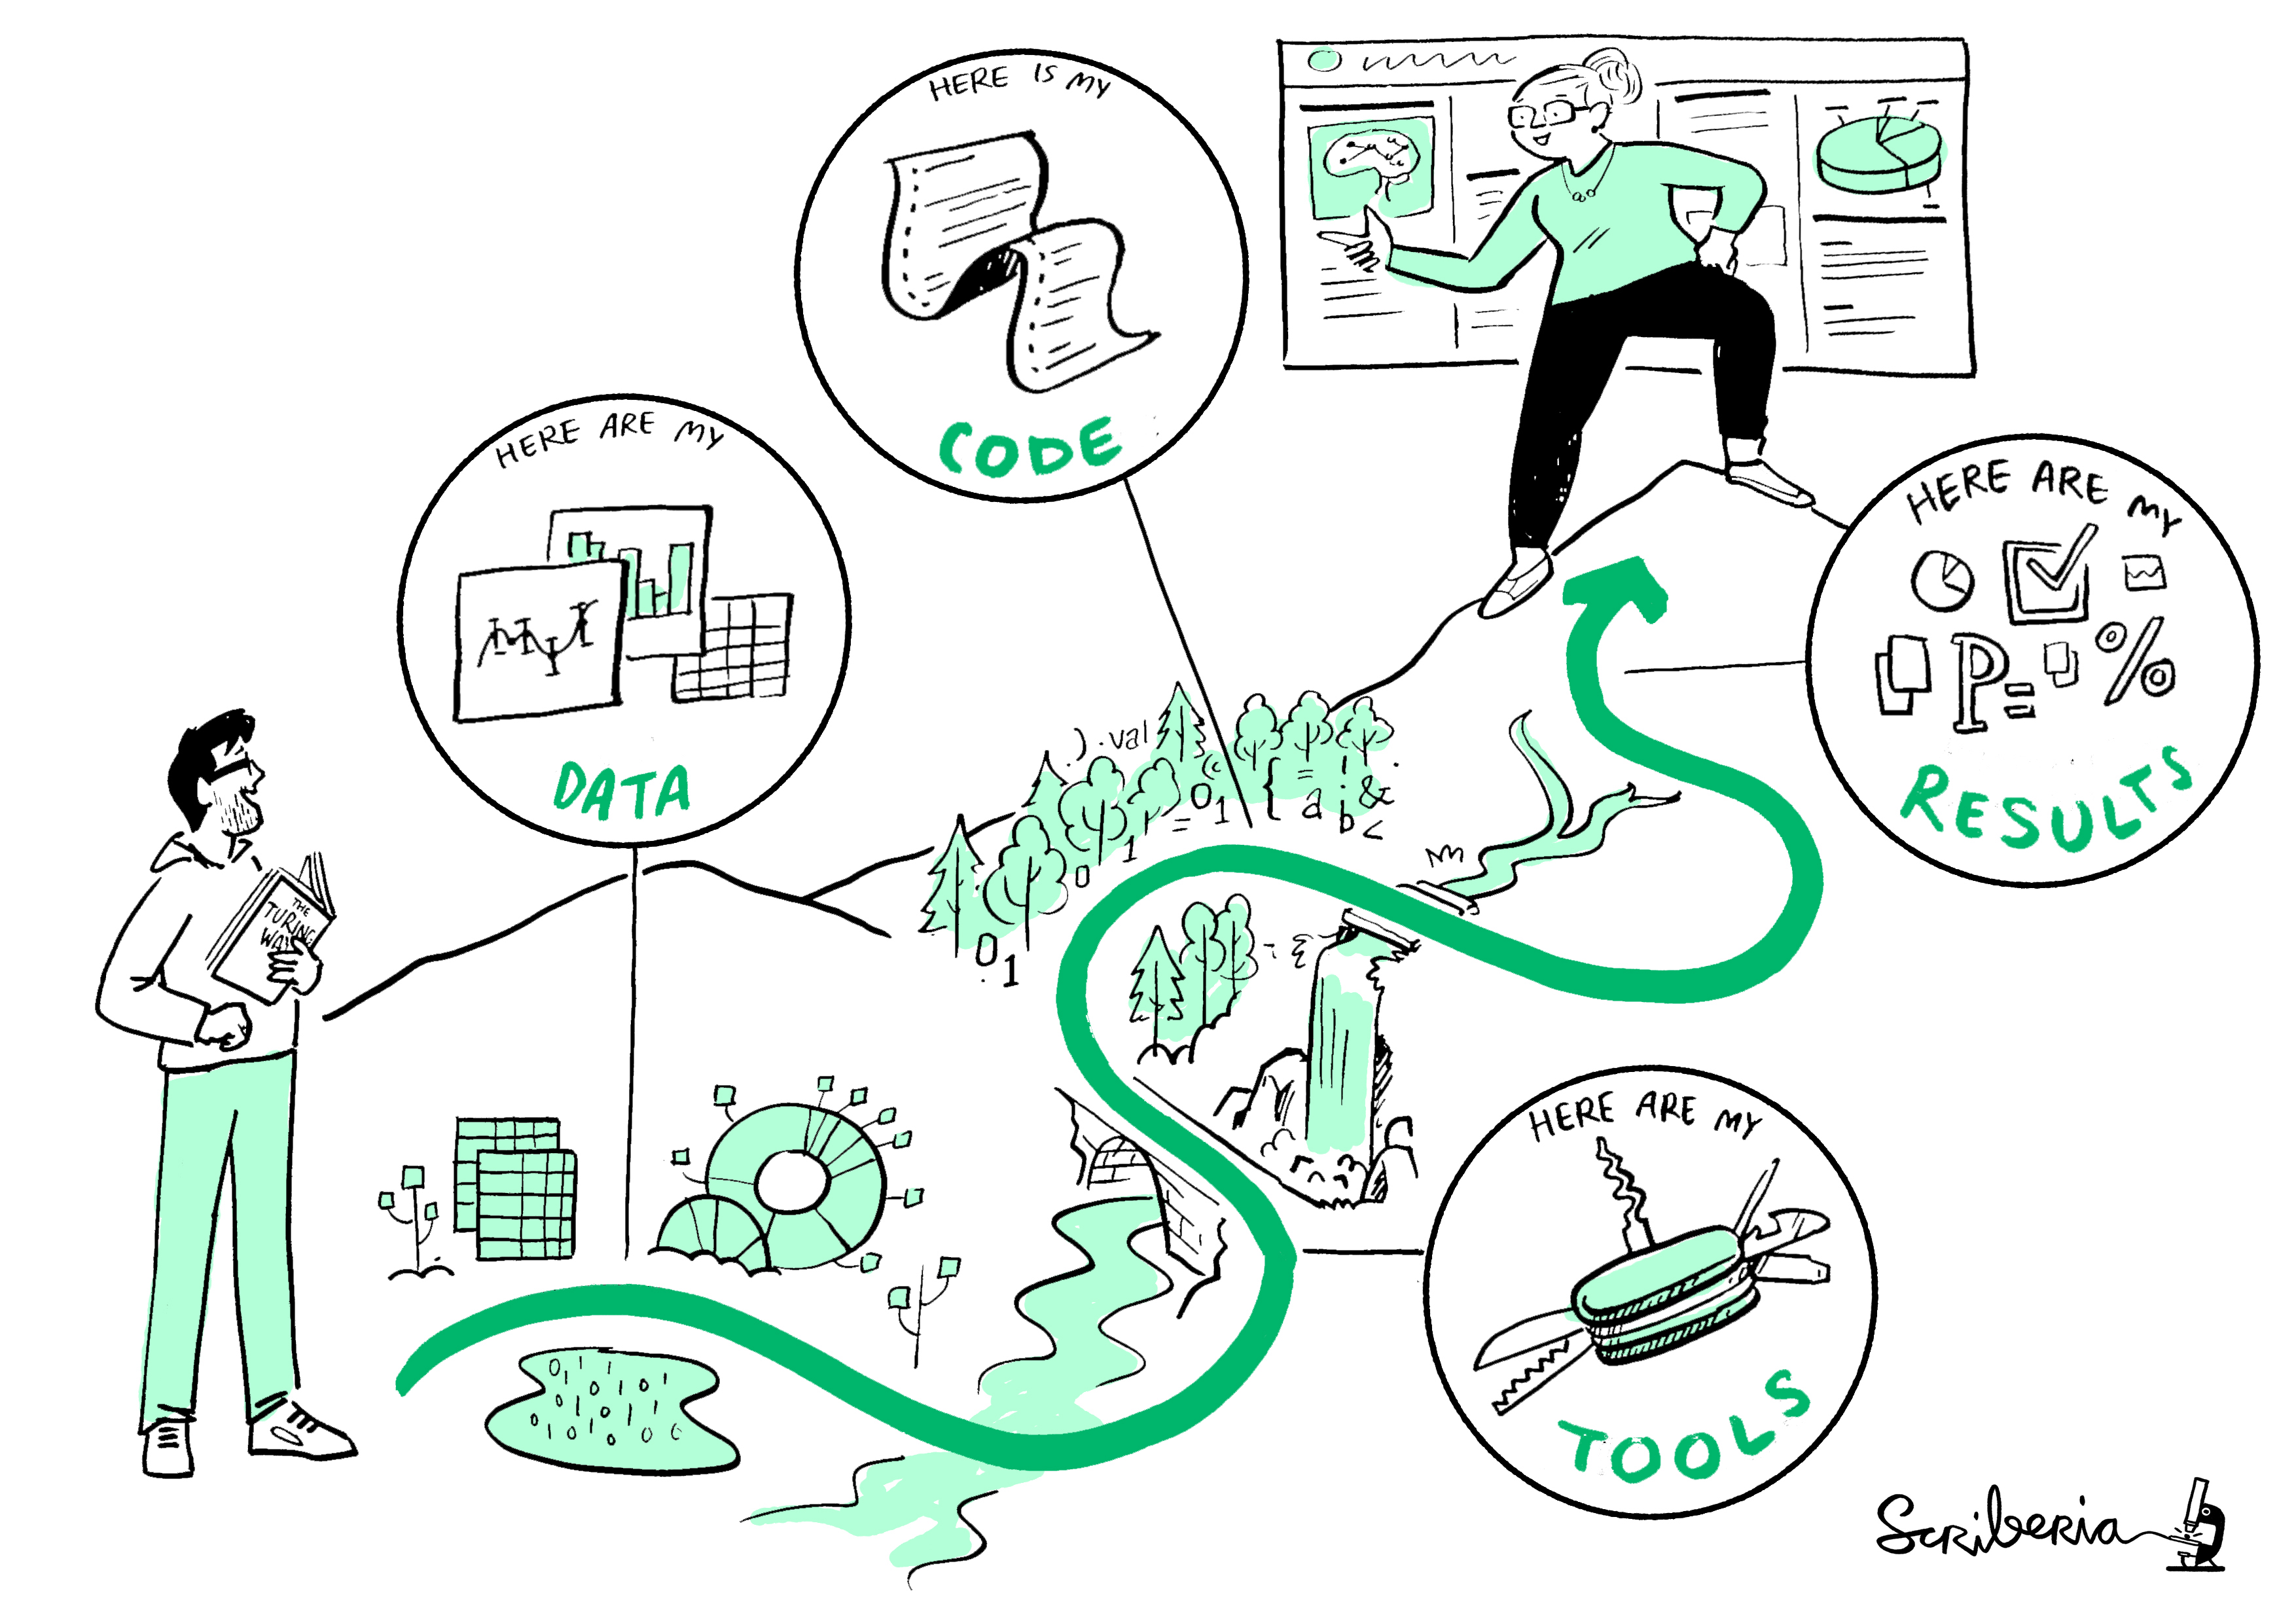
\includegraphics{rr-presentation-figure/ReproducibleJourney.jpg}

The need for reproducibility is increasing dramatically as data analyses become more complex and involve larger datasets, analysts, and more sophisticated computations.

\hypertarget{what-is-reproducible-research}{%
\section{what is reproducible research?}\label{what-is-reproducible-research}}

According to a U.S. National Science Foundation (NSF) subcommittee on replicability in science, ``reproducibility refers to the ability of a researcher to duplicate the results of a prior study using the same materials as were used by the original investigator. This entails that a result obtained by an experiment or observational study should be achieved again with a high degree of agreement when the study is replicated with the same methodology by different researchers

\hypertarget{terminology-distinctions}{%
\subsection{Terminology distinctions}\label{terminology-distinctions}}

Reproducible research is sometimes known as reproducibility, reproducible statistical analysis, reproducible data analysis, reproducible reporting, and literate programming.

\hypertarget{reproducible-versus-replicable}{%
\subsection{Reproducible versus replicable}\label{reproducible-versus-replicable}}

Replicability means obtaining consistent results across studies aimed at answering the same scientific question, each of which has obtained its own data.

\hypertarget{reproducible-versus-repeatable}{%
\subsection{Reproducible versus repeatable}\label{reproducible-versus-repeatable}}

Repeatability measures the variation in measurements taken by a single instrument or person under the same conditions, while reproducibility measures whether an entire study or experiment can be reproduced in its entirety.

This is a way for researchers to verify that their own results are true and are not just chance artifacts.

\hypertarget{reproducibility-crisis}{%
\subsection{Reproducibility crisis}\label{reproducibility-crisis}}

The replication crisis (or replicability crisis or reproducibility crisis) is, as of 2020, an ongoing methodological crisis in which it has been found that many scientific studies are difficult or impossible to replicate or reproduce. The replication crisis affects the social sciences and medicine most severely.

\hypertarget{the-problem-in-the-context-of-public-service}{%
\subsection{The problem in the context of public service}\label{the-problem-in-the-context-of-public-service}}

\begin{itemize}
\tightlist
\item
  Government is closed\\
\item
  The public doesn't know how decisions are made
\item
  Duplication of work within the government
\item
  Types of reproducibility
\end{itemize}

\hypertarget{the-solution-in-the-context-of-public-service}{%
\subsection{The solution in the context of public service}\label{the-solution-in-the-context-of-public-service}}

\begin{itemize}
\tightlist
\item
  Openness and transparency in government\\
\item
  Evidence based decision making\\
\item
  Efficiency\\
\item
  Enable others to use our methods or help improve ours
\end{itemize}

\hypertarget{barriers-to-open-and-reproducible-workflows}{%
\subsection{Barriers to open and reproducible workflows}\label{barriers-to-open-and-reproducible-workflows}}

\begin{itemize}
\tightlist
\item
  Directives\\
\item
  Approval of management\\
\item
  Data privacy and security policies\\
\item
  Culture
\end{itemize}

\hypertarget{what-needs-to-be-reproduced}{%
\subsection{What needs to be reproduced?}\label{what-needs-to-be-reproduced}}

For evidence-informed decision making, results need to be reproducible.

The results include:
- Stattistical and inferential tables
- Visualizations/figures/graphs
- Values reported in the text
- The statistical evidence in support of the findings (e.g., p-values, confidence intervals, credible intervals).

\hypertarget{motivation}{%
\subsection{Motivation}\label{motivation}}

Some aspects to consider that may make your experiments, processes, and reports more reproducible:
1. Don't Read Between the Lines. \ldots{}\\
2. Be Strict. \ldots{}\\
3. Keep Things Transparent. \ldots{}\\
4. Collaborate. \ldots{}\\
5. Automate Your Processes.

\hypertarget{benefits-of-reproducubility}{%
\section{Benefits of reproducubility}\label{benefits-of-reproducubility}}

\begin{itemize}
\tightlist
\item
  Increased likelihood that the research will be correct
\item
  Reproducibility makes it easier to check the research
\item
  It is easier to reproduce the research independently
\item
  Easier to extend the research
\item
  Reusable code and instruction resulting in increased efficiencies
\end{itemize}

\hypertarget{how-to-make-research-reproducible}{%
\section{How to make research reproducible}\label{how-to-make-research-reproducible}}

\begin{enumerate}
\def\labelenumi{\arabic{enumi})}
\tightlist
\item
  The first reason to repeat experiments is simply to verify results. Different science disciplines have different criteria for determining what good results are.
\item
  The next reason to repeat experiments is to develop skills necessary to extend established methods and develop new experiments. For these, we need reproducible methods, tools, and platforms.
\end{enumerate}

\hypertarget{requirements-for-reproducibility}{%
\section{Requirements for reproducibility}\label{requirements-for-reproducibility}}

\begin{enumerate}
\def\labelenumi{\arabic{enumi})}
\tightlist
\item
  The ``raw'' data is made available, where ``raw'' refers to the data prior to any manipulation by the researcher (e.g., prior to any data cleaning and transformation).
\item
  A complete set of instructions is provided explaining all steps used in the processing and analyzing the data.
\end{enumerate}

\hypertarget{additional-requirements}{%
\subsection{Additional requirements}\label{additional-requirements}}

\begin{enumerate}
\def\labelenumi{\alph{enumi})}
\item
  A set of files is provided containing the data and code, and it is possible to create the tables and any data-derived charts/graphics/visualizations by running the code.
\item
  Details about the system being used to run the analysis: operating system, patches, random number seeds, specific versions of all software/packages/libraries are listed.
\item
  The code is written in a way that can be readily understood.
\item
  Open/transparent. All the data and materials are available (as opposed to ``available upon request'') -- e.g., posted on GitHub, or in an international data repository.
\item
  That is, either:
\end{enumerate}

\begin{itemize}
\tightlist
\item
  Another party (e.g., a reviewer) has successfully reproduced the results and certified them as such.\\
\item
  Logs demonstrate that key results were successfully created from the inputs.\\
\item
  The key results are linked to the data and code, so the relationship can be directly inspected.
\end{itemize}

A final requirement, which is sometimes known as literate programming, is that:

\begin{enumerate}
\def\labelenumi{\alph{enumi})}
\setcounter{enumi}{5}
\tightlist
\item
  The entire report is written using code. That is, a file or files are provided which, when run, import the data, produce all the results, insert the results into the text of the report, and format the report.
\end{enumerate}

\hypertarget{tools-for-reproducible-projects}{%
\chapter{Tools for reproducible projects}\label{tools-for-reproducible-projects}}

``An article about computational science in a scientific publication is not the scholarship itself,
it is merely advertising of the scholarship. The actual scholarship is the complete software development environment and the complete set of instructions which generated the figures.''
--- Jonathan Buckheit and David Donoho, paraphrasing Jon Claerbout

``In 2002, I felt like I would just remember everything forever,'' Karl Broman, a biostatistician at the University of Wisconsin, Madison. ``It was only later that it became clear that you start to forget things within a month.''

\hypertarget{barriers}{%
\subsection{Barriers}\label{barriers}}

\begin{itemize}
\tightlist
\item
  Human subject data or proprietary code aren't shared and we need to implement creative solutions
\item
  Journals and funders don't reward reproducibility
\item
  Analysts need to be taught reproducible methodology and there is a steep learning curve
\item
  Need to make these efforts common place
\item
  Software changes, new versions are released and older code breaks.
\item
  Files are removed or moved and all the code breaks.
\item
  One file is updated but the rest of the code/files are not updated.
\item
  One forgets which files depend on which other files, or what has been changed
\end{itemize}

\hypertarget{tools}{%
\section{Tools}\label{tools}}

``Your primary collaborator is yourself 6 months from now, and your past self doesn't answer emails.'' - software carpentry

In this section, the tools that make reproducibility and open workflows easier are divided into four categories and these are not exhaustive. The categories include tools for data, methods, results, and communication products.

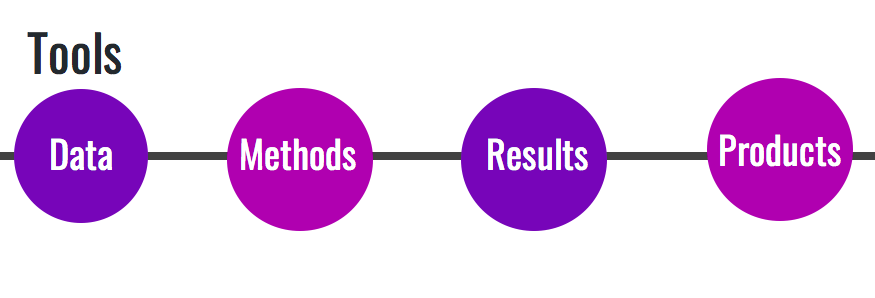
\includegraphics{rr-presentation-figure/tools.png}

The basics of research (data) management can be applied to every research project. These concepts include:
i) storing data carefully and securely (according to the appropriate standards in the case of sensitive data)\\
ii) backing up frequently and in at least two separate locations\\
iii) using a file naming convention so that others within and outside a project can understand a file's content.

\hypertarget{data}{%
\subsection{Data}\label{data}}

The question we can ask ourselves is how can we make the data FAIR: findable, accessible, interoperable, and reusable?

\begin{itemize}
\tightlist
\item
  Findable: e.g.~Make data available in trusted data repository\\
\item
  Accessible (store in open non-proprietary platforms/formats): e.g.~include comprehensive metadata
\item
  Interoperable (standardized and has identifiers): e.g.~store in open (non-proprietary) formats
\item
  Reusable (open with comprehensive metadata): For open data, attach a licence or rights waiver, or a permanent identifier (i.e.~DOI)
\end{itemize}

Some tools include:\\
- Shared drive/Local Area Network (LAN)/Sharepoint\\
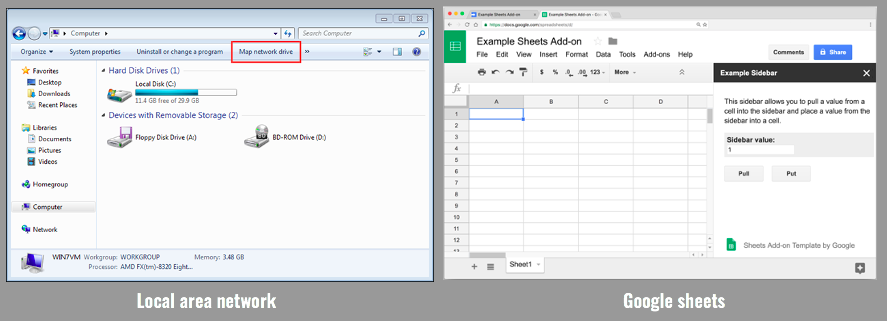
\includegraphics{rr-presentation-figure/LAN.png}

\begin{itemize}
\tightlist
\item
  Google sheets / OpenRefine\\
\item
  Open government portal\\
\item
  GitHub\\
  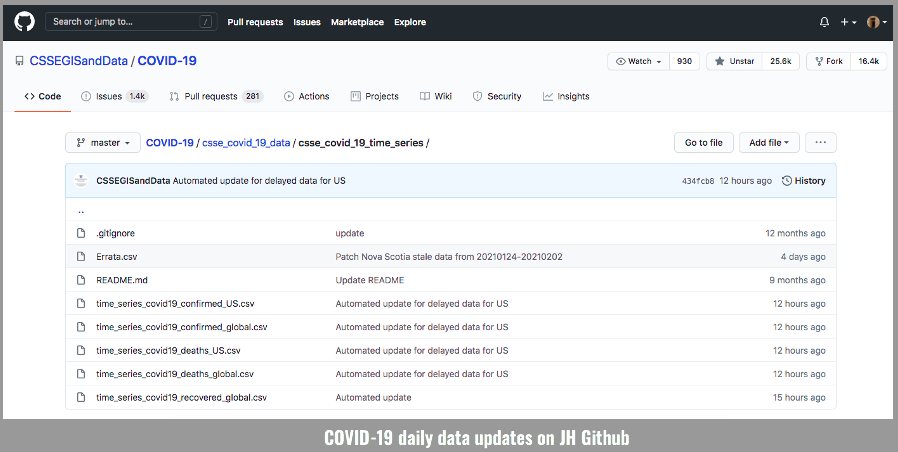
\includegraphics{rr-presentation-figure/Covid.png}
\end{itemize}

\hypertarget{methods}{%
\subsection{Methods}\label{methods}}

How can we make the process by which we do our work more open and reproducible? How could others access this work?

Some tools include:\\
- GCconnex\\
- Protocols.io

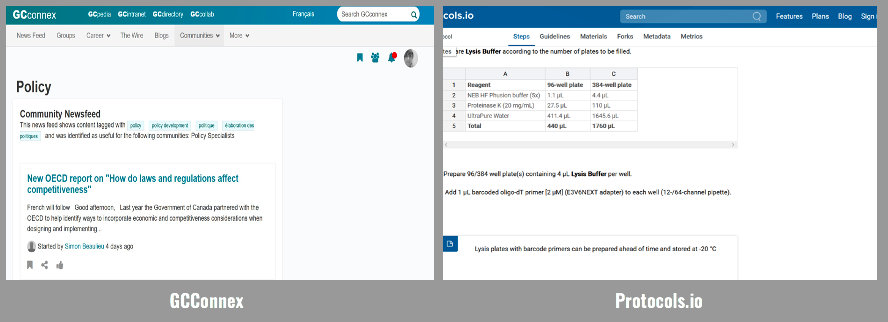
\includegraphics{rr-presentation-figure/methods.png}
- GitHub

\hypertarget{results}{%
\subsection{Results}\label{results}}

How can we adequately share the results with team members and tweak the methods to answer new questions/test new hypotheses?

Some tool examples include:\\
- Shared drive/LAN/Sharepoint and connection with respective analytic/data science softwares\\
- Google docs and other microsoft suites\\
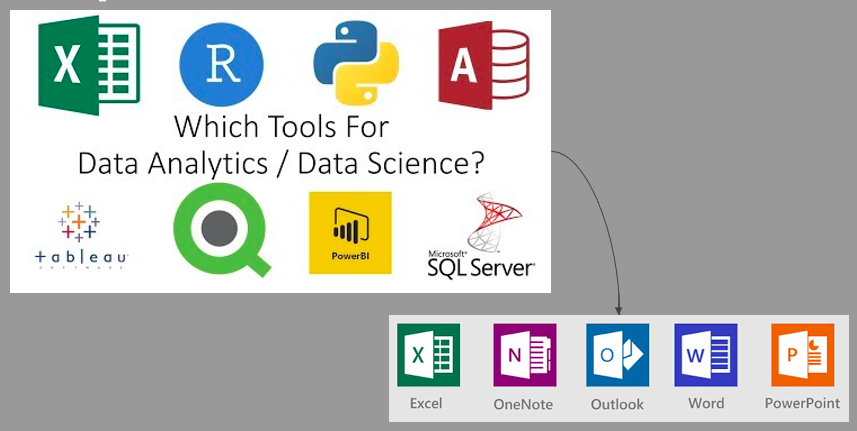
\includegraphics{rr-presentation-figure/results1.png}
- Github\\
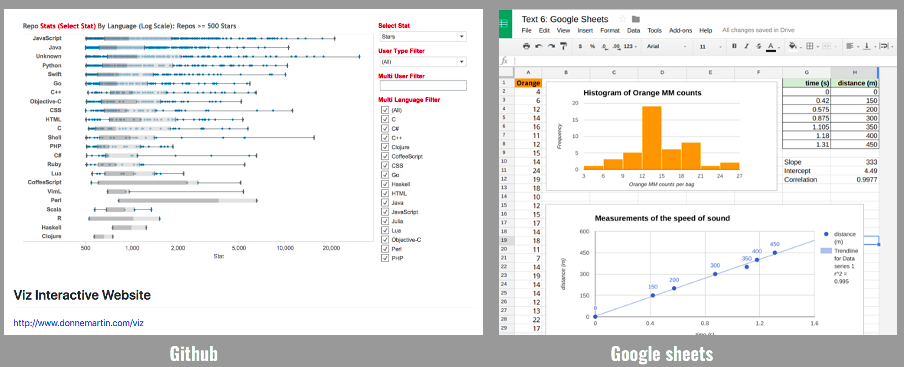
\includegraphics{rr-presentation-figure/results2.png}

\hypertarget{communication-products}{%
\subsection{Communication products}\label{communication-products}}

Once our work is done - how can we make it most accessible?

\begin{itemize}
\tightlist
\item
  Cochrane reports\\
\item
  Open access publications\\
\item
  Public talks\\
\item
  Media/Social Media\\
\item
  Github
\end{itemize}

Other considerations:\\
1. Share data, software, workflows, methods and results in open trusted repositories
2. Persistent links, permanent identifiers for data, code, digital artifacts upon which the results depend
3. Enable credit for shared digital scholarly objects with citations
4. Adequately document to facilitate reuse
5. Use Open Licensing
6. Journals should conduct a reproducibility check
7. Funding agencies should instigate new research programs and pilot studies

\texttt{Stodden,\ McNutt,\ Bailey,\ Deelman,\ Gil,\ Hanson,\ Heroux,\ Ioannidis,\ and\ Taufer\ (2016)\ in\ Science\ Policy\ Forum}

\hypertarget{giving-and-receiving-credits}{%
\chapter{Giving and receiving credits}\label{giving-and-receiving-credits}}

How do we make sure that others credit our work and we credit others?

We've often heard of Copyright, the authors' and composers' rights represented by the symbol ©.
It means All rights reserved therefore, we can't do anything with work that's copyright protected, unless we get permission directly from the author or composer, his or her representative (editor) or collective societies entrusted by authors and composers to manage their rights.

On the other hand, there exists the Copyleft, giving permission to anyone to copy, broadcast, use, modify and distribute work as long as some rights are reserved fairly. The author who chooses Copyleft lets other creators of the world know that they can do what they want with his or her work (within the limits of morality).

Although Copyright and Copyleft are on opposite sides of the spectrum, there are additional parameters we can use. For instance, Creative Commons, provides the spectrum and helps us legally share our knowledge and creativity to build a more equitable, accessible, and innovative world --- unlocking the full potential of the internet to drive a new era of development, growth and productivity.

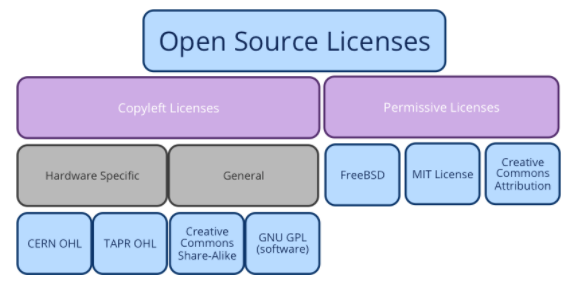
\includegraphics{rr-presentation-figure/rightleft.png}

Creative Commons lets you create licenses by choosing one or more permissions based on parameters like copying your work, modifying (remixing) it, sharing it, broadcasting it, distributing it, reusing it, and its attribution (giving due credit to its author). Different combinations are available.

\begin{itemize}
\item
  Open source code licences (MIT/Open Canada)
\item
  Information licences (Creative Commons)
  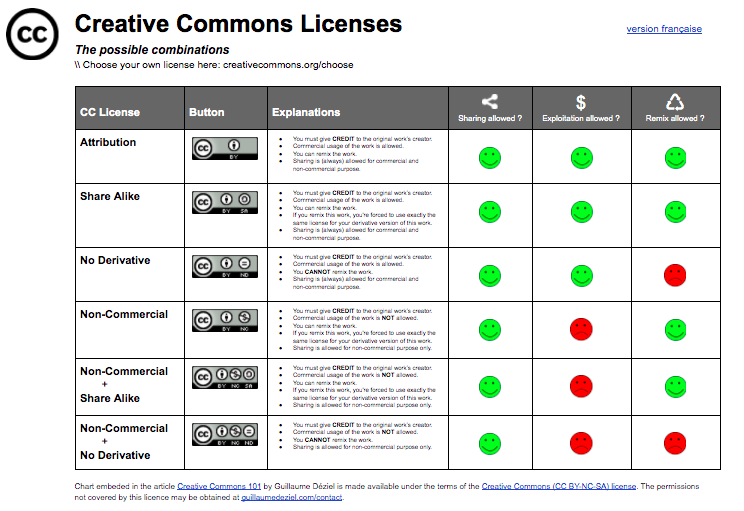
\includegraphics{rr-presentation-figure/cc.png}
\item
  Github (other examples can be found \href{https://2015.igem.org/Team:Cambridge-JIC/OpenHardwareRevolution}{here})
  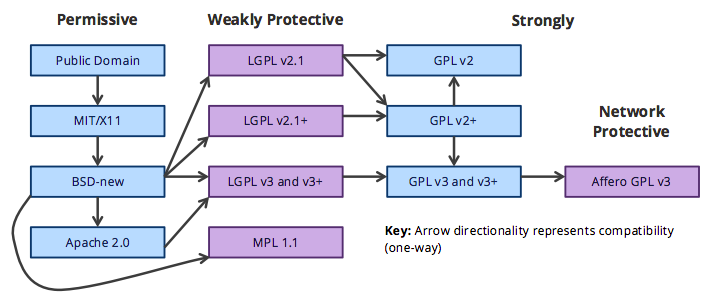
\includegraphics{rr-presentation-figure/opensource.png}
\end{itemize}

\hypertarget{introduction-to-markdown}{%
\chapter{Introduction to markdown}\label{introduction-to-markdown}}

\begin{itemize}
\tightlist
\item
  how does rmarkdown work? Advantages, disadvantages
\item
  rmarkdown syntax (examples)
\end{itemize}

\hypertarget{rmarkdown-and-usage}{%
\section{Rmarkdown and usage}\label{rmarkdown-and-usage}}

\begin{itemize}
\item
  reproducible reporting with rmarkdown
\item
  dichotomizing Rmarkdown document content to (1) computation component and (2) narrative component (\citet{MikeKane}, Yale) collectively called as research compendia
\item
  Research Compedia: a container for the different elements that make up the document and its computations (i.e.~text, code, data, \ldots) and as a means for distributing, managing, and updating the collection.
\end{itemize}

\hypertarget{computation-components}{%
\section{Computation components}\label{computation-components}}

\begin{itemize}
\tightlist
\item
  Objects to be presented: usually plots and tables
\item
  Reproducible code to visualize data
\end{itemize}

\hypertarget{narrative-components}{%
\section{Narrative components}\label{narrative-components}}

\begin{itemize}
\tightlist
\item
  Provide backgrounds, goals
\item
  Contexualize computational components
\item
  Establish themes
\item
  Convey the results
\item
  Render in pdf, html, docx
\end{itemize}

\hypertarget{rproject-set-up}{%
\section{Rproject set-up}\label{rproject-set-up}}

\begin{itemize}
\tightlist
\item
  Allows for integration of the two components (i.e.~creation of Rmarkdowns with compuational components)
\item
  Integrates literate programming
\item
  Provide interpretability and facilitate reproducibility
\end{itemize}

\hypertarget{demo}{%
\section{Demo}\label{demo}}

\begin{itemize}
\tightlist
\item
  End-to-end demonstration of a reproducible project
\item
  Please refer to \href{Beavers.Rmd}{Beaver.Rmd}
\end{itemize}

\hypertarget{git-commands}{%
\chapter{GIT Commands}\label{git-commands}}

\begin{itemize}
\tightlist
\item
  \protect\hyperlink{git-terminology}{GIT Terminology}
\item
  \protect\hyperlink{git-commands}{GIT Commands}
\item
  \protect\hyperlink{resources}{Resources}
\end{itemize}

\hypertarget{git-terminology}{%
\section{GIT Terminology}\label{git-terminology}}

\begin{itemize}
\item
  \texttt{origin} : connection pointing to the remote repository
\item
  \texttt{master} : name of your default branch. A branch in Git is simply a lightweight movable pointer to a commit
\item
  \texttt{working\ directory} : local repository
\item
  \texttt{.git\ directory} : Git stores all of its repository data in the .git directory. This is created when a local repository is initialised using the \texttt{init} command
\item
  \texttt{.git.ignore} : Git uses this file to determine which files and directories to ignore, before you make a commit
\item
  \texttt{hash}: the commit command creates a unique ID called a hash, which is an absolute path
\item
  \texttt{HEAD} : pointer to the last commit of the branch you are currently on. If you are on the master branch, then HEAD and master will refer to the same commit. This is a relative path. To see the previous commit use \texttt{HEAD\textasciitilde{}1}
\end{itemize}

\hypertarget{git-commands-1}{%
\section{GIT Commands}\label{git-commands-1}}

Initialise

\begin{itemize}
\tightlist
\item
  \texttt{git\ init\ \textless{}local\ repository\ name\textgreater{}}initialises a new local repository
\end{itemize}

Remotes

\begin{itemize}
\tightlist
\item
  \texttt{git\ remote\ add\ \textless{}remote\ name\textgreater{}\ \textless{}url\textgreater{}} creates a new connection to a remote repository is the shortcut for the and is typically set to `origin'
\item
  \texttt{git\ remote\ show\ \textless{}remote\ name\textgreater{}} shows which branch is automatically pushed to when you run git push while on certain branches. It also shows you which remote branches on the server you don't yet have, which remote branches you have that have been removed from the server, and multiple local branches that are able to merge automatically with their remote-tracking branch when you run git pull
\item
  \texttt{git\ remote\ rename\ \textless{}remote\ name\textgreater{}\ \textless{}new\ remote\ name\textgreater{}} rename a remote
\item
  \texttt{git\ remote\ remove\ \textless{}remote\ name\textgreater{}} remove a remote
\item
  \texttt{git\ remote\ -v} lists the remotes that are configured
\end{itemize}

Branches

\begin{itemize}
\tightlist
\item
  \texttt{git\ branch\ \textless{}new\ branch\ name\textgreater{}} adds a new branch, a structure with trees for saved states of files
\item
  \texttt{git\ checkout\ \textless{}branch\ name\textgreater{}\ \textless{}filename\textgreater{}} checks out (i.e.~switches to another version) an old version of a file
\item
  \texttt{git\ branch} lists all of the branches in a repository, with a * next to the branch you are currently on
\item
  \texttt{git\ checkout\ \textless{}branch-name\textgreater{}} switches to another branch-name
\item
  \texttt{git\ checkout\ -b\ branch-name\textgreater{}} creates the branch and switches you to it
\item
  \texttt{git\ merge\ source\ destination} merges two branches
\end{itemize}

Status

\begin{itemize}
\tightlist
\item
  \texttt{git\ status} shows which files have changed/new in your repository
\item
  \texttt{git\ diff} shows the changes you made to the file
\item
  \texttt{git\ diff\ -\/-staged} shows the difference between the last committed change and what's in the staging area
\item
  \texttt{git\ diff\ directory} shows the changes to the files in the directory
\item
  \texttt{git\ diff\ -r\ HEAD} -r flag refers to compare to a particular revision
\item
  \texttt{git\ log} view the log of the project's history
\item
  \texttt{git\ show\ \textless{}hash\textgreater{}} view the details of a specific commit, with the first few characters of the commit's hash
\item
  \texttt{git\ annotate\ \textless{}filename\textgreater{}} shows who made the last change to each line of a file and when
\end{itemize}

Clone

\begin{itemize}
\tightlist
\item
  \texttt{git\ clone\ \textless{}remote\ name\textgreater{}} to clone a repo and download a copy of a repo to a local folder This automatically creates the remote called origin
\end{itemize}

Add

\begin{itemize}
\tightlist
\item
  \texttt{git\ add} adds from your working directory to your staging area, ie specifies what will go in a snapshot
\item
  \texttt{git\ add\ \textless{}filename\textgreater{}} stages a file
\item
  \texttt{git\ add\ -A} stages all new, modified and deleted
\item
  \texttt{git\ add\ \textless{}foldername\textgreater{}/*} adds folder and contents to your staging area
\end{itemize}

Remove

\begin{itemize}
\tightlist
\item
  \texttt{git\ clean\ -n} shows a list of files that are in the repository, but whose history Git is not currently tracking
\item
  \texttt{git\ clean\ -f} will then delete those files
\end{itemize}

Undo

\begin{itemize}
\tightlist
\item
  \texttt{git\ reset} undo ALL changes that have been staged with git add
\item
  \texttt{git\ reset\ HEAD\ \textless{}filename\textgreater{}} undo changes to a specific filename that have been staged on HEAD
\end{itemize}

Commit

\begin{itemize}
\tightlist
\item
  \texttt{git\ commit\ -m\ "\textless{}message\textgreater{}"} commits the file with the snapshot to the \texttt{local\ repository} locally. The commit records the changes to the file ie actually takes the snapshot and makes a permanent record of it
\end{itemize}

Fetch

\begin{itemize}
\tightlist
\item
  \texttt{git\ fetch} gets any new work since last clone or fetch. Fetch does not however merge remote work with our work
\end{itemize}

Pull

\begin{itemize}
\tightlist
\item
  \texttt{git\ pull} automatically fetches and then merges that remote branch into your current branch
\end{itemize}

Push

\begin{itemize}
\tightlist
\item
  \texttt{git\ push} adds the files to your remote git
\end{itemize}

Note on adding files to the remote:

\begin{itemize}
\tightlist
\item
  When it is your first push from a repo, you will first have to make the link between the local and remote repository via: \texttt{git\ push\ \ -\/-set-upstream\ origin\ master}, or shorter \texttt{git\ push\ -u\ origin\ master}. As of then, \texttt{git\ push} will refer to the upstream branch you've set: i.e.~origin / master
\end{itemize}

\hypertarget{references}{%
\subsection{references}\label{references}}

\begin{itemize}
\tightlist
\item
  \href{http://happygitwithr.com/rmd-test-drive.html}{Happy Git and GitHub for the useR by Jennifer Bryan} adapted under \href{https://creativecommons.org/licenses/by/4.0/}{Creative Commons Attribution-NonCommercial 4.0 International License.}
\item
  \href{https://git-scm.com/book/en/v2}{Pro Git book, written by Scott Chacon and Ben Straub} adapted under the \href{https://creativecommons.org/licenses/by/3.0/}{Creative Commons Attribution Non Commercial Share Alike 3.0 license}
\item
  \href{http://swcarpentry.github.io/git-novice/}{Version Control with Git by Software Carpentry} adapted under the \href{https://creativecommons.org/licenses/by/4.0/}{Attribution 4.0 International (CC BY 4.0 license}
\end{itemize}

\hypertarget{resources}{%
\chapter{Resources}\label{resources}}

\hypertarget{blogs-sites-books-courses}{%
\section{(blogs, sites, books, courses):}\label{blogs-sites-books-courses}}

\begin{itemize}
\tightlist
\item
  Matthew Shotwell's slides (2011): \href{https://rstudio-pubs-static.s3.amazonaws.com/177032_7be0bffdc2274d679c03b7228ac7b91f.html}{``Approaches and Barriers to Reproducible Practices in Biostatistics''}
\item
  NIH Training Module: \href{https://grants.nih.gov/reproducibility/module_1/presentation.html}{Reproducibility through rigor and transparency}
\item
  Gandrud, Christopher. \href{https://englianhu.files.wordpress.com/2016/01/reproducible-research-with-r-and-studio-2nd-edition.pdf}{Reproducible Research with R and R Studio}, CRC Press, 2013.
\item
  Xie, Yihui. \href{http://static.latexstudio.net/wp-content/uploads/2014/03/DDR-Yihui-Xie-Chap1-3.pdf}{Dynamic Documents with R and knitr}, Vol. 29. CRC Press, 2013.
\item
  ROpenSci's blog post: \href{https://ropensci.org/blog/2014/06/09/reproducibility/}{``Reproducible research is still a challenge''}, by R. FitzJohn, M. Pennell, A. Zanne, W. Cornwell, June 9, 2014
\item
  Karl Broman's class \href{http://kbroman.org/Tools4RR/}{``Tools for Reproducible Research''} at UWisconsin-Madison.
\item
  ``Reproducible Research'' by Johns Hopkins on \href{https://www.coursera.org/learn/reproducible-research}{Coursera} (Peng, Leek, Caffo)
\item
  Stodden, Victoria, Friedrich Leisch, and Roger D. Peng, eds.~\href{https://www.jstatsoft.org/article/view/v061b02/v61b02.pdf}{Implementing reproducible research}, CRC Press, 2014.
\item
  StackOverflow question \href{https://stackoverflow.com/questions/1408450/why-should-i-use-version-control\#:~:text=Version\%20control\%20gives\%20you\%20the,using\%20tools.}{``Why should I use version control?''}
\item
  Learn git on github: \href{https://try.github.io/levels/1/challenges/1}{link}
\item
  Reproducible research with R and RStudio: \url{http://christophergandrud.github.io/RepResR-RStudio/}
\item
  Tools for reproducible research: \url{https://kbroman.org/Tools4RR/}
\item
  Data privacy and security: \url{https://dataprivacymanager.net/security-vs-privacy/}
\item
  BC-Gov framework for github \url{https://github.com/bcgov/BC-Policy-Framework-For-GitHub}
\item
  Making slides with Xaringan package in RMarkdown: \url{https://arm.rbind.io/slides/xaringan.html}
\item
  Data wrangling with R: \url{https://cengel.github.io/R-data-wrangling/}
\item
  Data cleaning with R and tidyverse: \url{https://towardsdatascience.com/data-cleaning-with-r-and-the-tidyverse-detecting-missing-values-ea23c519bc62}
\item
  Gallery of missing data visualization: \url{https://cran.r-project.org/web/packages/naniar/vignettes/naniar-visualisation.html}
\item
  How does R handle missing values: \url{https://stats.idre.ucla.edu/r/faq/how-does-r-handle-missing-values/}
\item
  What does research reproducibility mean? \url{https://stm.sciencemag.org/content/8/341/341ps12}
\item
  Challenge to scientists: does your ten-year-old code still run? \url{https://www.nature.com/articles/d41586-020-02462-7?utm_source=twitter\&utm_medium=social\&utm_content=organic\&utm_campaign=NGMT_USG_JC01_GL_Nature\#ref-CR1}
\item
  Reproducible Research and open science: \url{https://ropensci.github.io/reproducibility-guide/sections/introduction/}
\end{itemize}

\hypertarget{participant-polls}{%
\section{Participant polls}\label{participant-polls}}

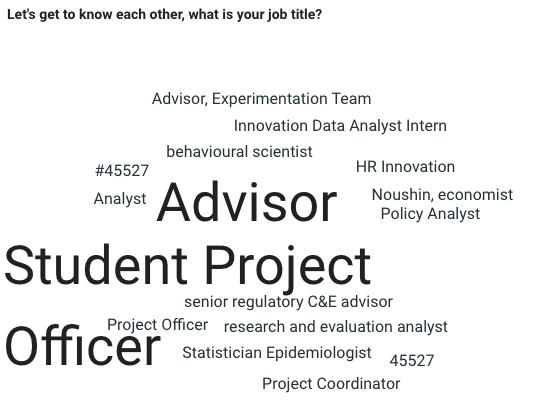
\includegraphics{rr-presentation-figure/Q1.png}
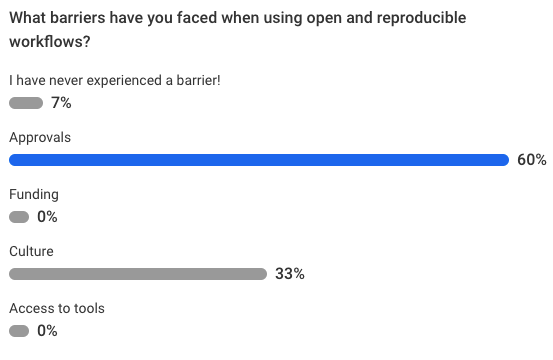
\includegraphics{rr-presentation-figure/Q2.png}
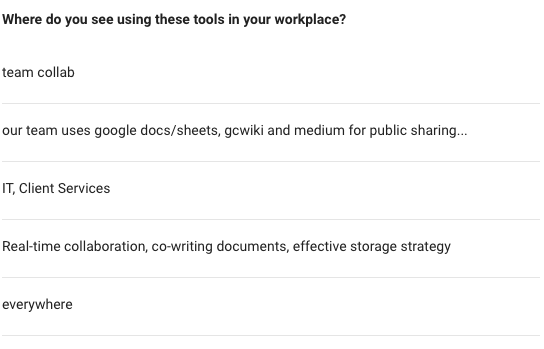
\includegraphics{rr-presentation-figure/Q3.png}

\end{document}
